\chapter{Trajectory Plot}
\label{appx:simulation}

\newpage

\begin{figure}[H]
	\centering
	\begin{tikzpicture}
		
		% Main trajectory image
		\node[anchor=south west, inner sep=0] (main) at (0,0)
		{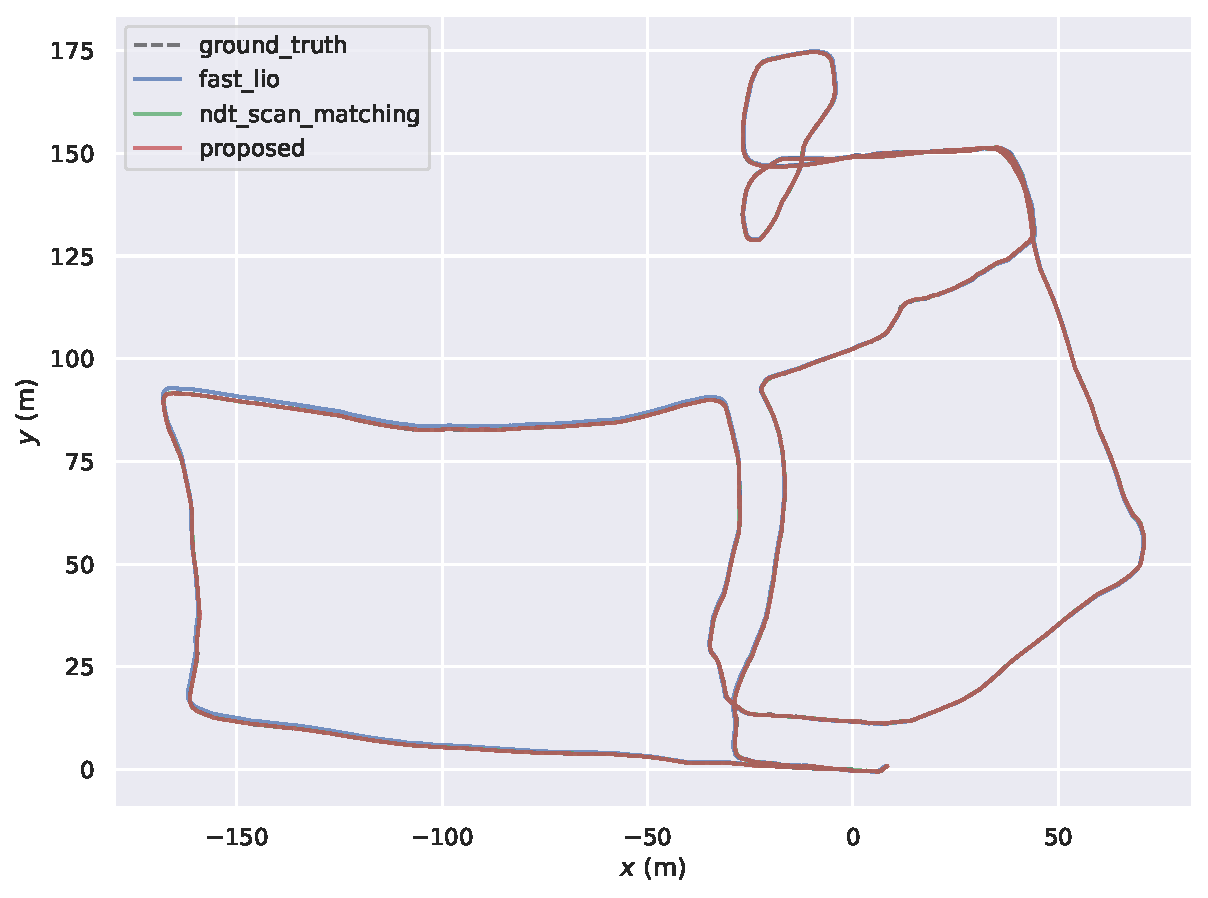
\includegraphics[width=1\textwidth]{images/trajectory_plot_seq2.pdf}};
		% Coordinate system normalized to the image
		\begin{scope}[x={(main.south east)}, y={(main.north west)}]
			% Red dashed rectangle for zoom box (adjust coordinates!)
			\draw[red, thick, dashed] (0.1, 0.45) rectangle (0.25, 0.6);
			% Red arrow from zoom box to zoomed-in image
			\draw[->, red, thick] (0.25, 0.6) -- (.265, 0.65);
		\end{scope}
		
		% Zoomed-in image overlay (use exact x/y in cm to place)
		\node[anchor=south west] at (4.43, 6.8)
		{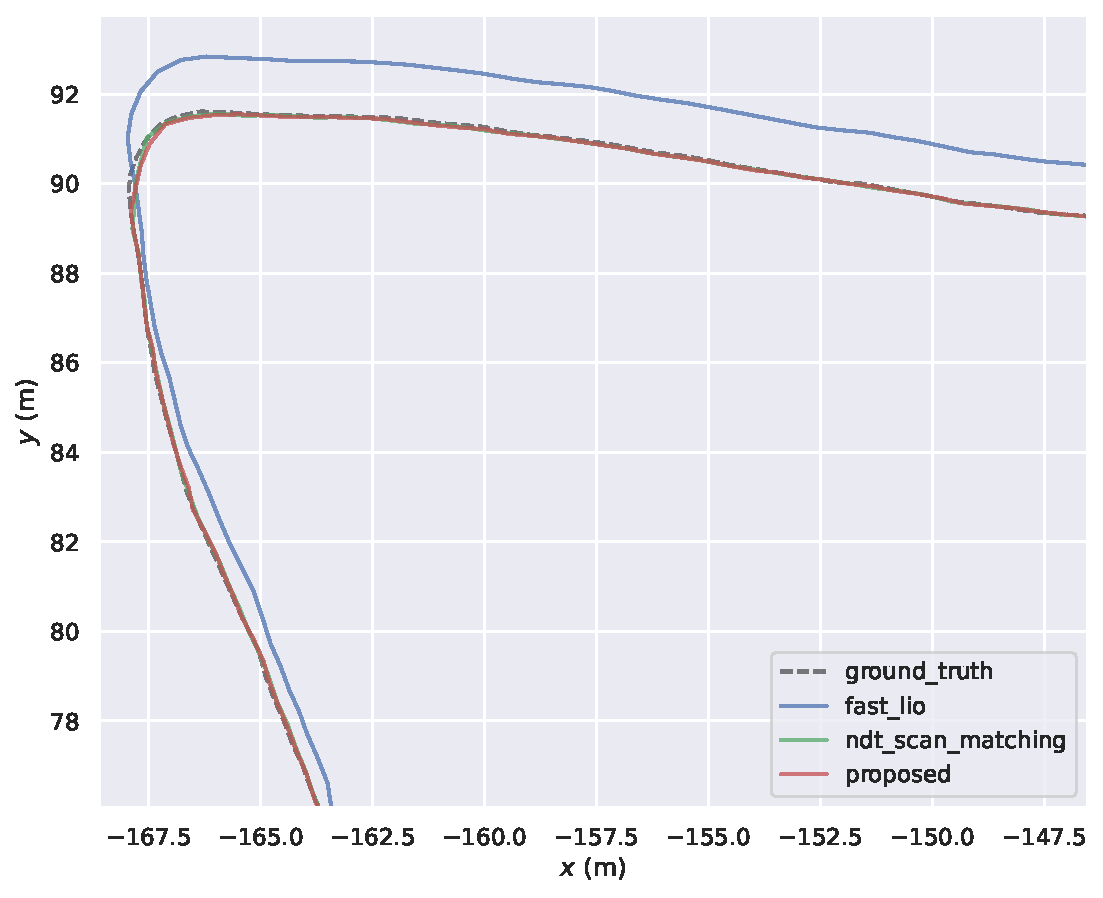
\includegraphics[width=0.335\textwidth]{images/trajectory_plot_zoom_seq2.pdf}};
		
		% Optional label
		%\node at (15, 4.6) {\small Zoomed-in detail};
		
	\end{tikzpicture}
	\caption[Saxion Sequence 02– Trajectory Alignment with Zoomed Comparison]%
	{\textbf{Saxion Sequence 02 – Trajectory Alignment.} 
		The figure shows the estimated trajectories from FAST-LIO2, low frequency NDT map matching , and the proposed method, overlaid against ground truth. The red dashed box indicates the zoomed region.
	}
	\label{fig:saxion-seq2-trajectory-zoom}
	
	
\end{figure}

\begin{figure}[H]
	\centering
	\begin{tikzpicture}
		
		% Main trajectory image
		\node[anchor=south west, inner sep=0] (main) at (0,0)
		{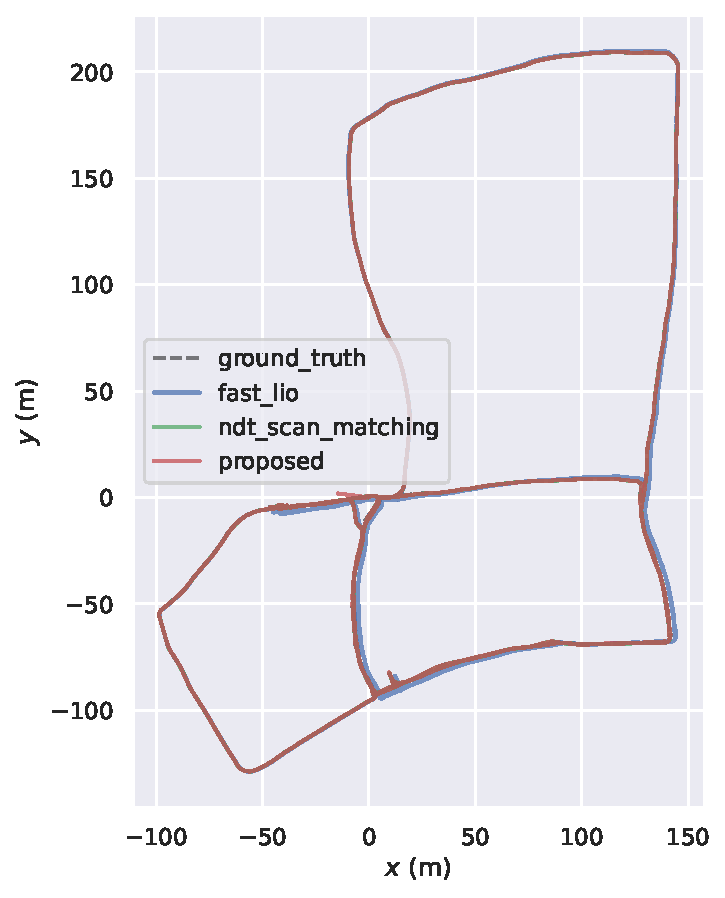
\includegraphics[width=0.92\textwidth]  {images/trajectory_plot_seq3.pdf}};
		% Coordinate system normalized to the image
		\begin{scope}[x={(main.south east)}, y={(main.north west)}]
			% Red dashed rectangle for zoom box (adjust coordinates!)
			\draw[red, thick, dashed] (0.8, 0.4) rectangle (0.95, 0.5);
			% Red arrow from zoom box to zoomed-in image
			\draw[->, red, thick] (0.8, 0.45) -- (0.47, 0.7);
		\end{scope}
		
		% Zoomed-in image overlay (use exact x/y in cm to place)
		\node[anchor=south west] at (0.22, 11.6)
		{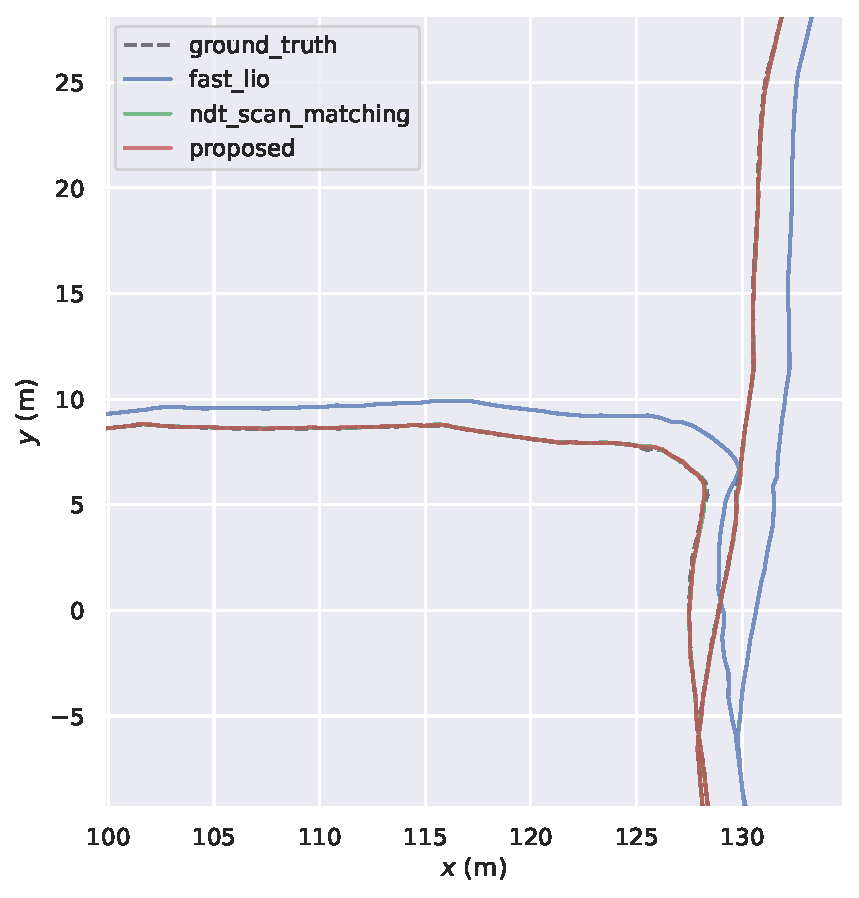
\includegraphics[width=0.4\textwidth]{images/trajectory_zoom_seq3.pdf}};
		
		% Optional label
		%\node at (15, 4.6) {\small Zoomed-in detail};
		
	\end{tikzpicture}
	
\caption[Saxion Sequence 03 – Trajectory Alignment with Zoomed Comparison]%
{\textbf{Saxion Sequence 03 – Trajectory Alignment.} 
	The figure shows the estimated trajectories from FAST-LIO2, low frequency NDT map matching , and the proposed method, overlaid against ground truth. The red dashed box indicates the zoomed region.
}
\label{fig:saxion-seq3-trajectory-zoom}
\end{figure}


\begin{figure}[H]
	\centering
	\begin{subfigure}[t]{0.46\textwidth}
		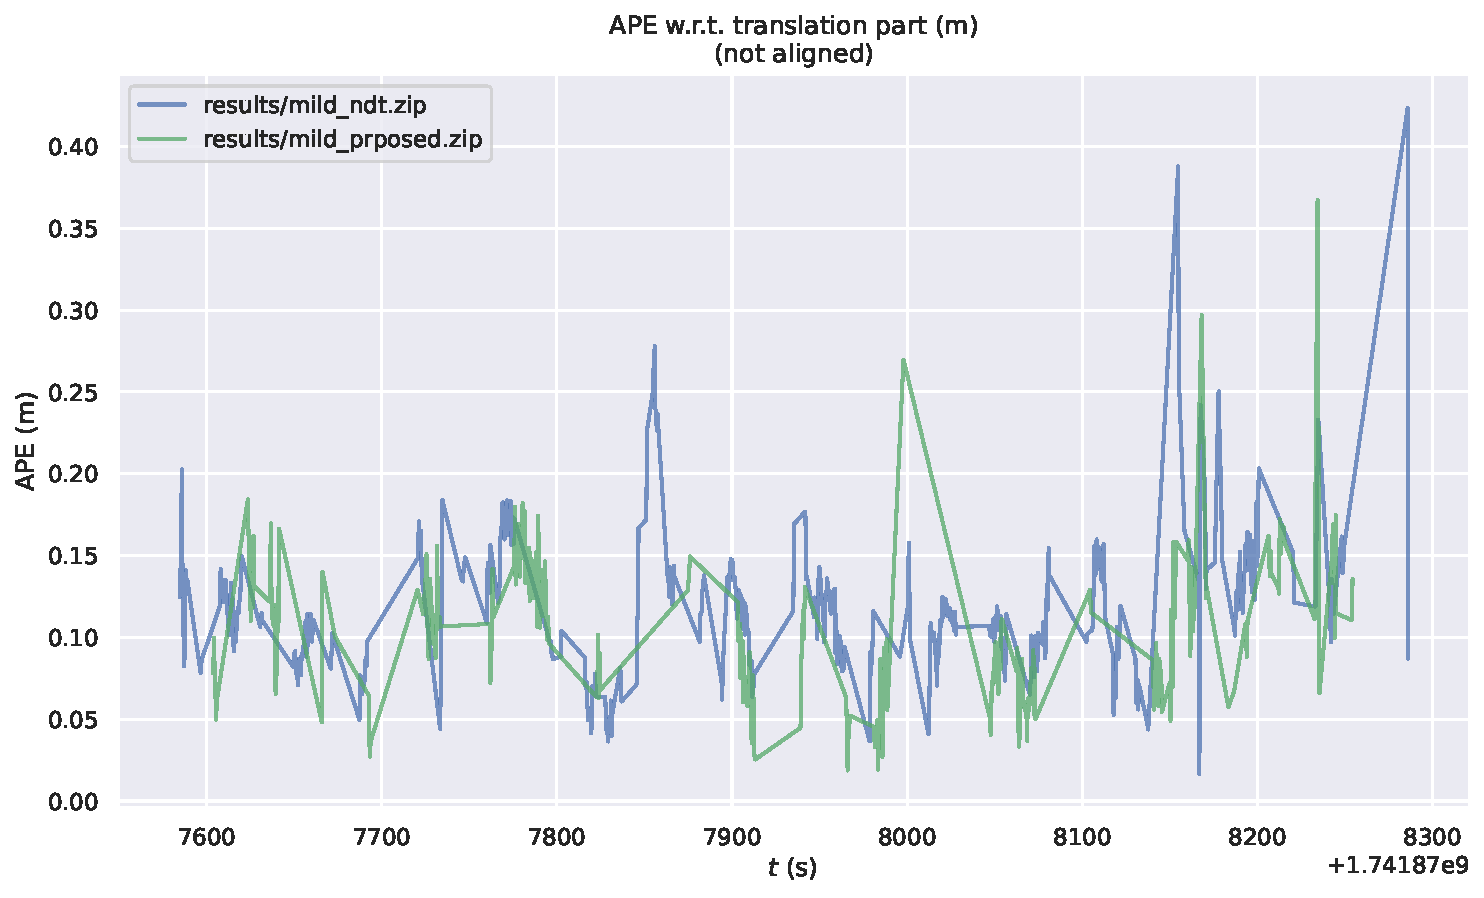
\includegraphics[  width=\linewidth]{images/mild.pdf}
		\caption{ Mild noise level ATE}
		\label{fig:mild-noise-level-pointcloud}
	\end{subfigure}
	\hfill
	\begin{subfigure}[t]{0.46\textwidth}
		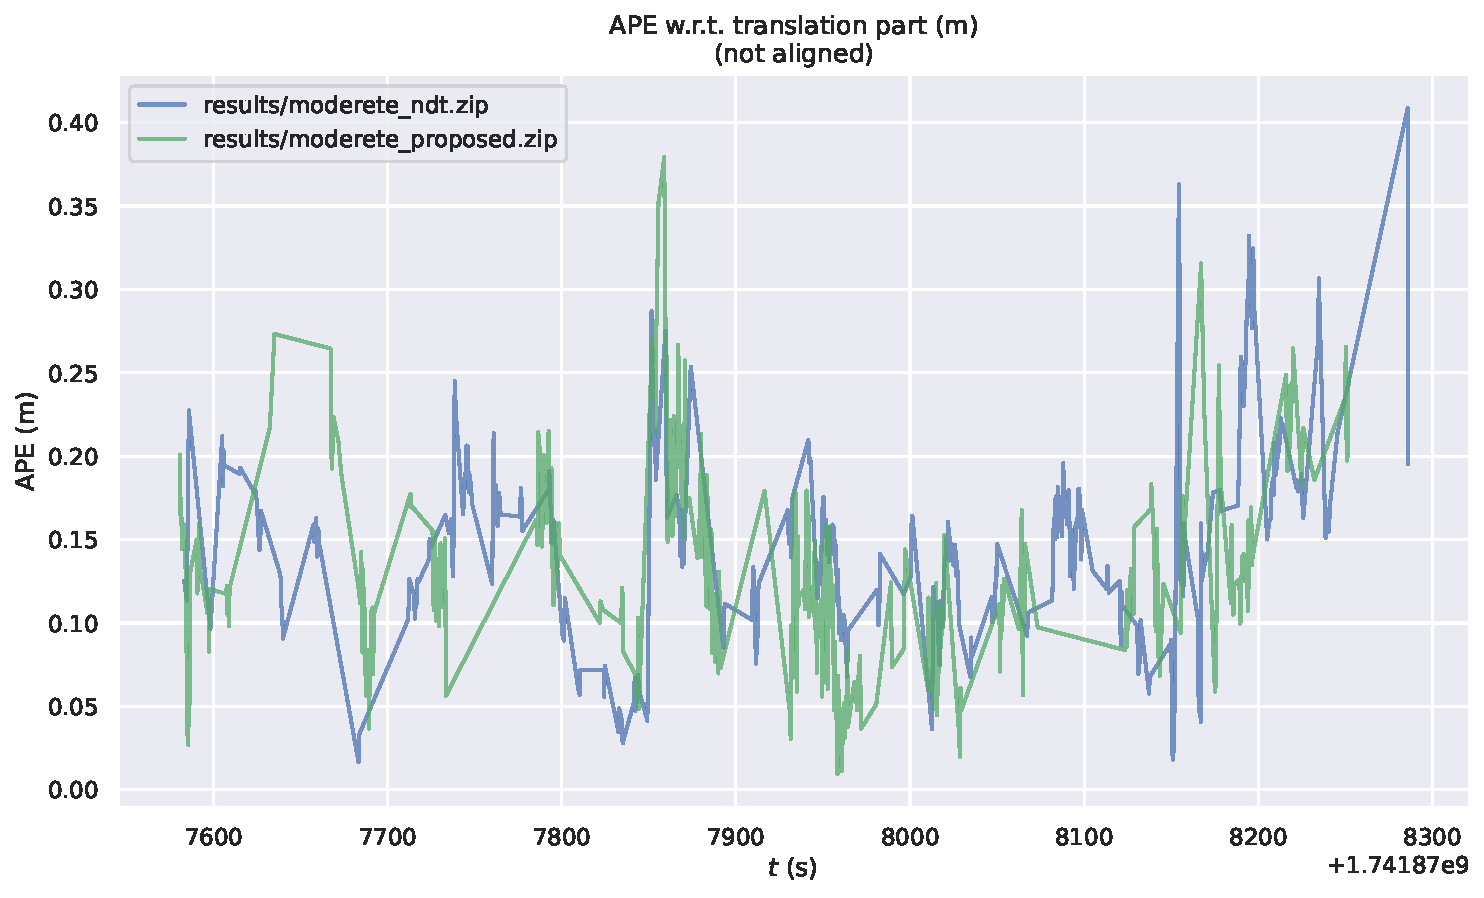
\includegraphics[width=\linewidth]{images/moderete.pdf}
		\caption{ Moderate noise level ATE error
		}
		\label{fig:moderete-noise-level-ate}
	\end{subfigure}
	\hfill
	\begin{subfigure}[t]{0.46\textwidth}
		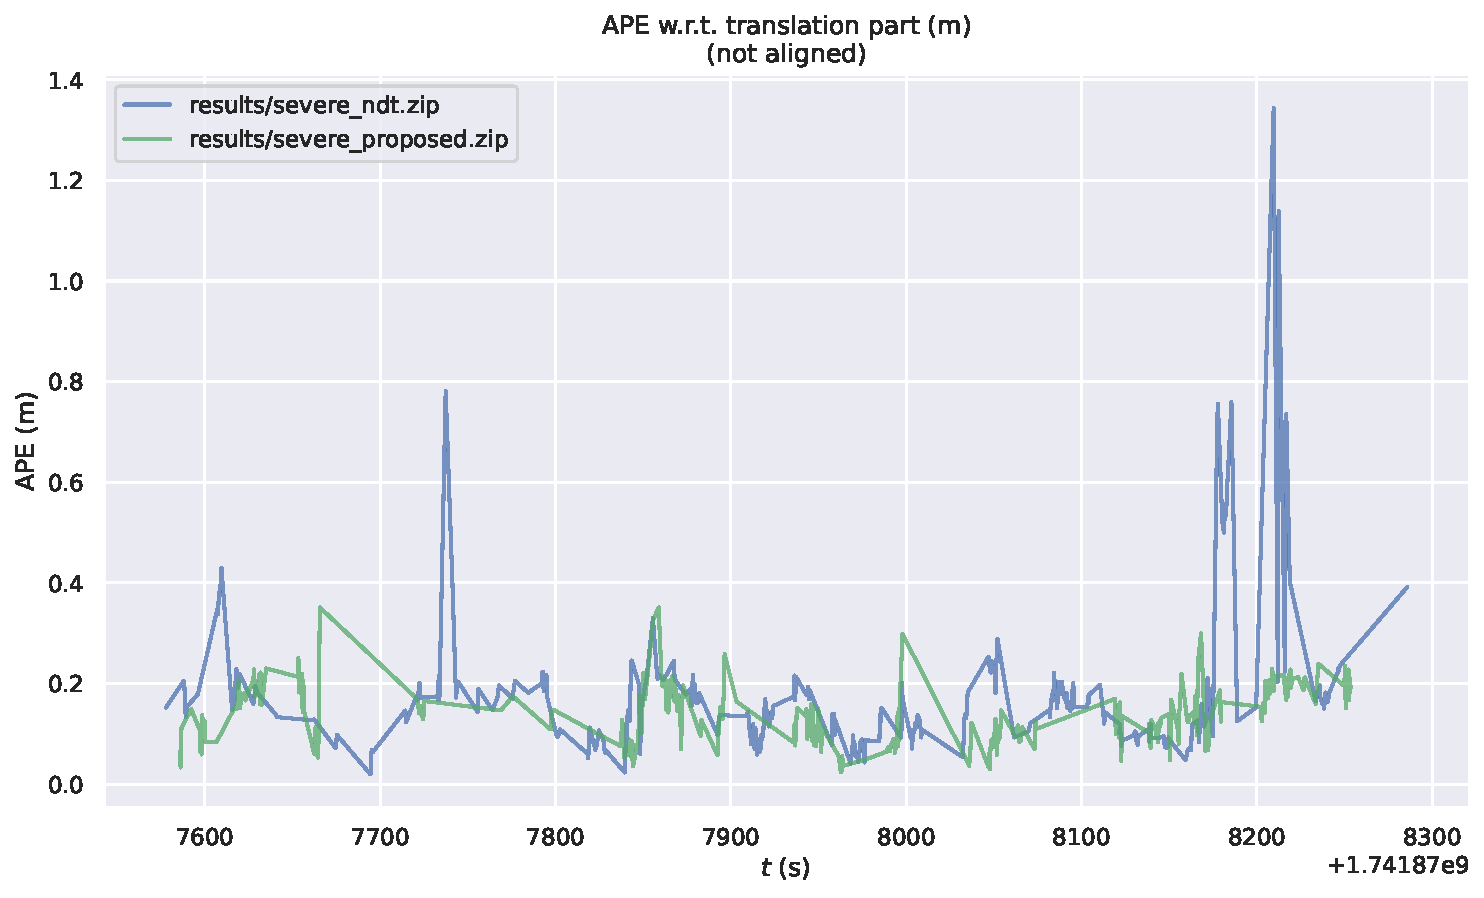
\includegraphics[ width=\linewidth]{images/severe.pdf}
		\caption{ Severe noise level ATE error
		}
		\label{fig:severe-noise-level-ate}
	\end{subfigure}
	
	\caption{NDT scan matching and proposed Translation (APE) Error statistics under Mild, Moderate, and Severe
		composite noise (b) Mild noise; (c) Moderate noise; (d) Severe noise.}
	
	\label{fig:different-noise-levels-ate}
\end{figure}


